\documentclass[a4paper,12pt]{article}

% ── Encoding ──────────────────────────────────────────────────────────────────
\usepackage[T1]{fontenc}
\usepackage[utf8]{inputenc}

% ── Font: Times New Roman equivalent ──────────────────────────────────────────
\usepackage{mathptmx}          % Times New Roman for body + math

% ── Page Layout: reduced margins for a larger text block ──────────────────────
\usepackage[a4paper, left=0.6in, right=0.6in, top=0.6in, bottom=0.6in]{geometry}

% ── Line Spacing: 1.15 ────────────────────────────────────────────────────────
\usepackage{setspace}
\setstretch{1.15}

% ── Paragraph spacing ─────────────────────────────────────────────────────────
\usepackage{parskip}
\setlength{\parindent}{0pt}
\setlength{\parskip}{6pt}

% ── Section Heading Fonts: 14pt bold ──────────────────────────────────────────
\usepackage{titlesec}
\titleformat{\section}
  {\normalfont\fontsize{14}{17}\bfseries}{\thesection}{1em}{}
\titleformat{\subsection}
  {\normalfont\fontsize{13}{16}\bfseries}{\thesubsection}{1em}{}
\titleformat{\subsubsection}
  {\normalfont\fontsize{12}{15}\bfseries}{\thesubsubsection}{1em}{}

% ── Figures & Captions ────────────────────────────────────────────────────────
\usepackage{graphicx}
\usepackage{float}
\usepackage[
  labelfont=bf,
  textfont=it,
  justification=centering,
  skip=6pt
]{caption}

% ── Tables ────────────────────────────────────────────────────────────────────
\usepackage{booktabs}
\usepackage{array}

% ── Equations (auto-numbered) ─────────────────────────────────────────────────
\usepackage{amsmath}
\usepackage{amssymb}

% ── TikZ Graphics ──────────────────────────────────────────────────────────────
\usepackage{tikz}
\usetikzlibrary{shapes,arrows,positioning,calc,fit}

% ── Code Listings: Courier New 10pt ───────────────────────────────────────────
\usepackage{listings}
\usepackage{xcolor}

\lstset{
  basicstyle      = \fontfamily{pcr}\selectfont\fontsize{10}{12}\selectfont,
  keywordstyle    = \bfseries\color{blue!70!black},
  commentstyle    = \itshape\color{gray},
  stringstyle     = \color{orange!80!black},
  numberstyle     = \tiny\color{gray},
  numbers         = left,
  numbersep       = 8pt,
  stepnumber      = 1,
  frame           = single,
  framerule       = 0.4pt,
  rulecolor       = \color{black!30},
  backgroundcolor = \color{gray!5},
  breaklines      = true,
  breakatwhitespace = true,
  showstringspaces  = false,
  tabsize         = 4,
  captionpos      = b,
}

% ── Hyperlinks ────────────────────────────────────────────────────────────────
\usepackage[
  colorlinks = true,
  linkcolor  = black,
  citecolor  = black,
  urlcolor   = blue
]{hyperref}

% ── Table of Contents ─────────────────────────────────────────────────────────
\usepackage{tocloft}
\setcounter{tocdepth}{3}
\renewcommand{\cftsecleader}{\cftdotfill{\cftdotsep}}
\renewcommand{\cftsubsecleader}{\cftdotfill{\cftdotsep}}

% ── Misc ──────────────────────────────────────────────────────────────────────
\usepackage{microtype}
\usepackage{url}

% =============================================================================
\begin{document}

% ── Title Page ────────────────────────────────────────────────────────────────
\begin{titlepage}
  \centering
  \vspace*{0.6cm}

  {\Large\bfseries INDIAN INSTITUTE OF TECHNOLOGY TIRUPATI}\\[0.3cm]
  {\large\bfseries Department of Mechanical Engineering}\\[1.4cm]

  {\large\bfseries ME316L -- CAD-CAM}\\[0.2cm]
  {\Large\bfseries Course Project Report}\\[1.0cm]

  {\LARGE\bfseries NURBS Surface Modeler}\\[0.25cm]
  {\Large\bfseries with G-Code Export}\\[1.4cm]

  {\large\bfseries Project 10}\\[1.6cm]

  {\large\bfseries Submitted By}\\[0.6cm]

  \begin{tabular}{>{\bfseries}l >{\bfseries}l}
    ME22B040 & PULIPATI SAICHANDRA KUMAR       \\[4pt]
    ME23B036 & NIRANJAN M                      \\[4pt]
    ME23B028 & MAGHAM RAM CHARAN               \\[4pt]
    ME22B011 & BODDU NAGA VENKATA GIRISH       \\
  \end{tabular}

  \vfill
  % {\small\bfseries Indian Institute of Technology Tirupati}\\[0.2cm]
  {\small\bfseries Academic Year 2025--2026}
\end{titlepage}

\clearpage

% ── Table of Contents ─────────────────────────────────────────────────────────
\renewcommand{\contentsname}{\Large\bfseries Contents}
\tableofcontents
\clearpage

% =============================================================================
\section{Objectives}

\begin{enumerate}
    \item To implement a tensor-product NURBS surface $\mathbf{S}(u,v)$ from a
          user-defined $m \times n$ control net with per-point weights.
    \item To build an interactive 3-D GUI in Python using \texttt{PyQt} for the
          interface and \texttt{PyVista} for real-time rendering of the surface
          and control net.
    \item To compute surface normals via partial derivatives
          $\partial\mathbf{S}/\partial u$ and $\partial\mathbf{S}/\partial v$
          at any parameter point $(u,v)$.
    \item To generate a zig-zag 3-axis CNC toolpath offset along the surface
          normal by tool radius $R$, with chord-tolerance filtering
          ($\delta < 0.01$\,mm).
    \item To export a valid G-code file with correct header (\texttt{G21},
          \texttt{G90}, \texttt{M3}, \texttt{M8}), rapid moves, feed moves,
          and \texttt{M30} end-of-program.
\end{enumerate}

% =============================================================================
\section{Introduction}

NURBS (Non-Uniform Rational B-Spline) surfaces are fundamental mathematical
tools in CAD/CAM applications, enabling the representation of both analytical
and free-form geometries within a unified parametric framework~\cite{ref1}.
The tensor-product NURBS representation offers superior flexibility for
surface design and interpolation, making it particularly valuable for CNC
machining applications where smooth, predictable toolpaths are essential for
achieving high-quality surface finishes~\cite{ref2}.

In CNC manufacturing, the conversion from geometric design to machine-ready
code involves several critical steps: (1)~curve and surface construction using
spline primitives, (2)~surface evaluation at discrete parameter points,
(3)~computation of surface normals for tool orientation, (4)~generation of
offset toolpaths accounting for tool radius, and (5)~filtering and
optimization to produce valid G-code commands~\cite{ref3}. This project
integrates these steps into an interactive desktop application combining
real-time 3D visualization with comprehensive CNC programming capabilities.

A NURBS surface of degree $(p, q)$ is defined as
\begin{equation}
  \mathbf{S}(u,v) =
    \frac{\displaystyle\sum_{i=0}^{n}\sum_{j=0}^{m}
          N_{i,p}(u)\,N_{j,q}(v)\,w_{ij}\,\mathbf{P}_{ij}}
         {\displaystyle\sum_{i=0}^{n}\sum_{j=0}^{m}
          N_{i,p}(u)\,N_{j,q}(v)\,w_{ij}},
  \label{eq:nurbs}
\end{equation}
where $\mathbf{P}_{ij}$ are the $m \times n$ array of control points in
three-dimensional space, $w_{ij}$ are positive scalar weights associated with
each control point, and $N_{i,p}(u)$, $N_{j,q}(v)$ are the B-spline basis
functions of degree $p$ and $q$ in the $u$ and $v$ parameter directions,
respectively~\cite{ref1}. The weights enable the rational representation,
allowing the exact representation of conic sections and other important
analytical shapes. The use of uniform knot vectors with clamped endpoints
ensures that the surface passes through the boundary control points, a
property particularly valuable for edge definition in machined surfaces.

% =============================================================================
\section{Methodology}

\subsection{System Architecture}

The NURBS Surface Modeller is structured as a modular Python application
comprising six principal components: (1)~\emph{core/} for curve representations
and B-spline basis function evaluation using the Cox-de Boor recursion,
(2)~\emph{surface/} for tensor-product NURBS surface evaluation and generation,
(3)~\emph{machining/} for toolpath computation with normal offsets and
collinearity filtering, (4)~\emph{gcode/} for CNC G-code synthesis from
toolpath data, (5)~\emph{gui/} for interactive PyQt5-based visual design and
operation control, and (6)~\emph{utils/} for geometric utility functions
(vector normalization, cross products, distance calculations).

The data flow pipeline is: \emph{GUI input} $\rightarrow$ \emph{curve
management} $\rightarrow$ \emph{surface generation} $\rightarrow$
\emph{toolpath computation} $\rightarrow$ \emph{G-code export}. Users interact
with the application through a collapsible section interface organizing
functionality into six groups: (i)~Curves (creation, type selection, editing),
(ii)~Control Point Editor (direct XYZ/weight manipulation), (iii)~Surface
Generation (method and parameter selection), (iv)~Surface Operations
(extrusion and offset modes), (v)~Toolpath Generation (scanning parameters,
tool configuration), and (vi)~G-Code Export (CNC machine settings). The GUI
maintains state synchronization throughout the workflow, with PyVista
providing real-time 3D visualization of curves, surfaces, control nets, and
toolpath data.

\begin{figure}[H]
  \centering
  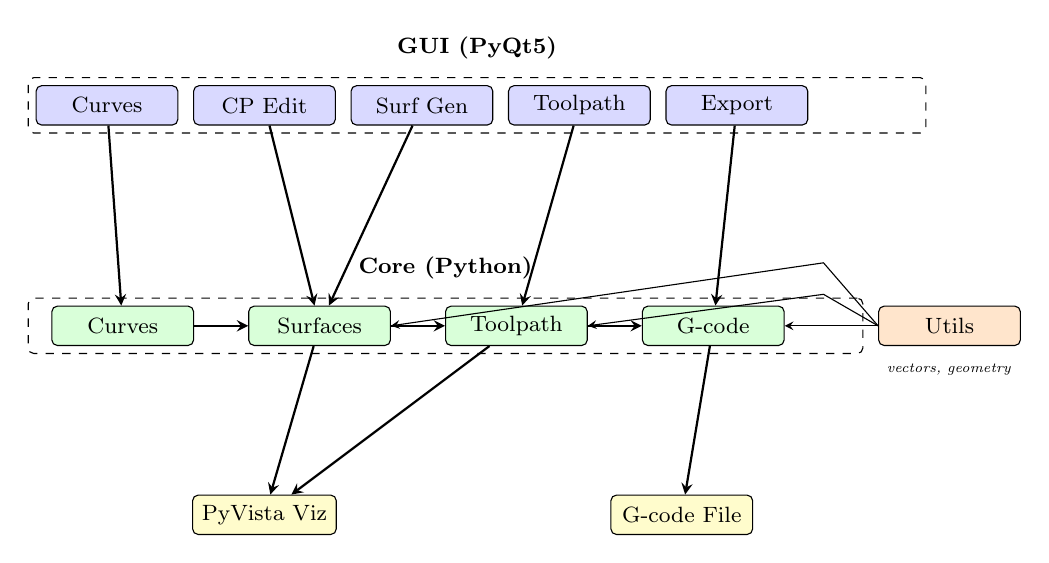
\begin{tikzpicture}[
    box/.style={rectangle, draw, rounded corners=2pt, minimum width=1.8cm,
                minimum height=0.5cm, align=center, font=\footnotesize},
    arrow/.style={->, >=stealth, thick},
    thin_arrow/.style={->, >=stealth, thin},
    layer/.style={rectangle, draw=black, dashed, rounded corners=2pt,
                  inner sep=10pt}
  ]

  % User Interface Layer
  \node[layer, minimum width=11.4cm] (ui_layer) at (5.7, 5.8) {};
  \node[box, fill=blue!15] (curves_ui) at (1.0, 5.8) {Curves};
  \node[box, fill=blue!15] (cpeditor) at (3.0, 5.8) {CP Edit};
  \node[box, fill=blue!15] (surfgen) at (5.0, 5.8) {Surf Gen};
  \node[box, fill=blue!15] (toolpath_ui) at (7.0, 5.8) {Toolpath};
  \node[box, fill=blue!15] (export) at (9.0, 5.8) {Export};
  \node[above=3pt of ui_layer, font=\footnotesize] {\textbf{GUI (PyQt5)}};

  % Core Computation Layer
  \node[layer, minimum width=10.6cm] (comp_layer) at (5.3, 3.0) {};
  \node[box, fill=green!15] (crv_core) at (1.2, 3.0) {Curves};
  \node[box, fill=green!15] (surf_core) at (3.7, 3.0) {Surfaces};
  \node[box, fill=green!15] (toolpath_core) at (6.2, 3.0) {Toolpath};
  \node[box, fill=green!15] (gcode_core) at (8.7, 3.0) {G-code};
  \node[above=3pt of comp_layer, font=\footnotesize] {\textbf{Core (Python)}};

  % Support Utilities (side column)
  \node[box, fill=orange!20] (utils) at (11.7, 3.0) {Utils};
  \node[below=3pt of utils, font=\tiny] {\textit{vectors, geometry}};

  % Output Layer
  \node[box, fill=yellow!20] (pyvista) at (3.0, 0.6) {PyVista Viz};
  \node[box, fill=yellow!20] (output) at (8.3, 0.6) {G-code File};

  % UI to Core: Vertical arrows
  \draw[arrow] (curves_ui) -- (crv_core);
  \draw[arrow] (cpeditor) -- (surf_core);
  \draw[arrow] (surfgen) -- (surf_core);
  \draw[arrow] (toolpath_ui) -- (toolpath_core);
  \draw[arrow] (export) -- (gcode_core);

  % Core pipeline: Main data flow
  \draw[arrow] (crv_core) -- (surf_core);
  \draw[arrow] (surf_core) -- (toolpath_core);
  \draw[arrow] (toolpath_core) -- (gcode_core);

  % Utils connections: Routed from the side to avoid overlap
  \draw[thin_arrow] (utils.west) -- (10.1, 3.0) -- (gcode_core.east);
  \draw[thin_arrow] (utils.west) -- (10.1, 3.4) -- (toolpath_core.east);
  \draw[thin_arrow] (utils.west) -- (10.1, 3.8) -- (surf_core.east);

  % Core to Output
  \draw[arrow] (surf_core) -- (pyvista);
  \draw[arrow] (toolpath_core) -- (pyvista);
  \draw[arrow] (gcode_core) -- (output);

  \end{tikzpicture}
  \caption{System architecture showing modular organization and data flow from
           GUI through core computation modules to visualization and file output.
           Utils provides support functions to core components.}
  \label{fig:blockdiagram}
\end{figure}

\subsection{Curve Representations and B-Spline Basis Functions}

The application supports three primary curve types: Bezier curves, uniform
B-spline curves, and NURBS curves. Each shares a common interface for
evaluation and derivative computation, enabling flexible curve composition.

\emph{Bezier curves} use the de Casteljau algorithm for stable point
evaluation: given a curve parameter $t \in [0, 1]$ and control points
$\mathbf{P}_0, \ldots, \mathbf{P}_n$, the algorithm recursively computes
intermediate points via linear interpolation, achieving $O(n^2)$ complexity.
Bezier curves are evaluated directly without knot vectors, making them
computationally efficient for low-degree segments.

\emph{B-spline and NURBS curves} rely on basis function evaluation via the
Cox-de Boor recursion~\cite{ref2}. For a parameter value $u$, the algorithm
first locates the knot span index $k$ satisfying $u_k \le u < u_{k+1}$ using
binary search ($O(\log n)$), then evaluates all degree-$p$ basis functions
$N_{i,p}(u)$ for relevant control points ($O(p^2)$ operations):
\begin{align}
  N_{i,0}(u) &= \begin{cases}
    1 & \text{if } u_i \le u < u_{i+1} \\
    0 & \text{otherwise}
  \end{cases}, \\
  N_{i,p}(u) &= \frac{u - u_i}{u_{i+p} - u_i} N_{i,p-1}(u) +
    \frac{u_{i+p+1} - u}{u_{i+p+1} - u_{i+1}} N_{i+1,p-1}(u).
\end{align}
Division-by-zero cases are handled gracefully (evaluating the fraction as~0).
The cumulative complexity for curve evaluation at $m$ parameter points is thus
$O(m(\log n + p^2))$. First derivatives are computed similarly, enabling
tangent vector and acceleration computations for curve analysis.

All basis function computations employ clamped uniform knot vectors with
Epsilon tolerance ($\epsilon = 10^{-10}$) for numerical stability.

\begin{figure}[H]
  \centering
  
\includegraphics[width=0.85\textwidth]{assets/2.png}
  \caption{GUI interface for curve creation and manipulation. Shows the viewport
           with rendered curve (blue polyline) and control points (red/blue spheres),
           alongside the Curves Panel with type selector, degree spinner, and
           control point list editor.}
  \label{fig:curve_editing_gui}
\end{figure}

\subsection{NURBS Surface Construction}

NURBS surfaces are represented as tensor products of two parametric curves,
with the control net stored as an $m \times n \times 3$ array and weights as
an $m \times n$ array. The surface is evaluated at a parameter pair $(u, v)$
by computing the double sum in Eq.~\eqref{eq:nurbs} using homogeneous
coordinates: each control point $\mathbf{P}_{ij} = (x_{ij}, y_{ij}, z_{ij})$
is converted to $(w_{ij} x_{ij}, w_{ij} y_{ij}, w_{ij} z_{ij}, w_{ij})$,
double-summed with basis functions, then projected back to 3D by dividing the
first three coordinates by the weight (fourth coordinate). This technique
achieves $O((p^2 + q^2) \log(mn))$ complexity while maintaining numerical
robustness.

Surface derivatives are computed using the quotient rule on the homogeneous
representation, allowing precise computation of surface normals via the
cross product:
\begin{equation}
  \mathbf{n}(u, v) = \frac{\partial \mathbf{S}}{\partial u} \times
    \frac{\partial \mathbf{S}}{\partial v}.
\end{equation}
Surface normals are essential for both visualization and toolpath offset
computation, as they define the direction of tool advancement relative to the
surface.

% \begin{figure}[H]
%   \centering
%   \fbox{\parbox{0.85\textwidth}{\centering\vspace{3.2cm}
%         \textit{Placeholder: NURBS surface visualization in PyVista showing
%                  the rendered surface mesh (shaded gray), control net
%                  (red wireframe polyhedron), control points (blue vertices),
%                  and coordinate axes.}
%         \vspace{3.2cm}}}
%   \caption{NURBS surface visualization showing the parametric surface mesh
%            with overlaid control net and control points. The surface is
%            rendered with transparency to reveal the underlying control structure.}
%   \label{fig:surface_visualization}
% \end{figure}

\begin{figure}[H]
  \centering
  
\includegraphics[width=0.85\textwidth]{assets/4.png}
  \caption{GUI panel for surface generation control. Users select surface
           creation method and adjust parameters. The Generate Surface button
           triggers surface construction and visualization.}
  \label{fig:surface_generation_panel}
\end{figure}

The application provides five distinct surface generation methods to accommodate
diverse design workflows:
\begin{enumerate}
  \item \textbf{Loft from Curves}: Constructs a surface interpolating multiple
    input curves (profiles). Each curve is sampled at uniform parameter
    intervals, and corresponding points across profiles are connected with
    linear B-splines. Ideal for transitioning between geometric cross-sections.

  \item \textbf{Linear Extrusion}: Sweeps a base curve along a constant
    direction vector, generating a ruled surface. The two-parameter NURBS
    representation uses the original curve parameters in one direction and a
    linear parameter ($0$ to $1$) in the extrusion direction.

  \item \textbf{Surface Normal Extrusion}: Offsets a base surface along its
    computed normal vector at each parameter point. Given offset distance $d$,
    each point $(u, v)$ is moved to $\mathbf{S}(u, v) + d \cdot \mathbf{n}(u, v)$.
    Particularly valuable for designing adjacent surfaces in multi-pass machining.

  \item \textbf{Surface Body Extrusion (Solid Mode)}: Generates triangulated
    surface bodies from NURBS surfaces. The entire enclosed volume is
    discretized, enabling ray-casting-based toolpath computation.

  \item \textbf{Surface Body Extrusion (Shell Mode)}: Generates a hollow shell
    representation suitable for visualization and containment queries during
    toolpath filtering.
\end{enumerate}

\subsection{Toolpath Generation and Normal Offset}

Toolpath generation converts the NURBS surface representation into a sequence
of discrete contact and center-line (CL) points suitable for CNC machine
execution. The algorithm employs a zigzag scanning pattern:

\begin{enumerate}
  \item \textbf{Parameter Grid Generation}: The surface is scanned at discrete
    $v$-parameter intervals (determined by the stepover distance and surface
    span). At each $v$ value, the $u$ parameter is varied from $0$ to $1$ at
    discrete intervals.

  \item \textbf{Contact Point Determination}: For each $(u, v)$ pair, the
    surface point $\mathbf{S}(u, v)$ is computed as the contact point. The
    surface normal $\mathbf{n}(u, v)$ is computed and normalized to unit
    length.

  \item \textbf{Center-Line Offset}: The tool center-line (CL) point is
    computed as
    \begin{equation}
      \mathbf{CL}(u, v) = \mathbf{S}(u, v) + r \cdot \mathbf{n}(u, v),
    \end{equation}
    where $r$ is the tool radius. This offset ensures that the rotating tool
    tip follows the intended surface profile.

  \item \textbf{Collinearity Filtering}: Sequential toolpath points that are
    nearly collinear (deviation $< 0.05~\text{mm}$) are removed to reduce
    redundant moves. This filtering preserves geometric fidelity while
    minimizing code length and execution time.

  \item \textbf{Pass Organization}: The complete toolpath is organized into
    passes, each corresponding to a fixed $v$ parameter. Passes alternate
    direction (forward/backward $u$ scanning) to minimize rapid (non-cutting)
    movements.
\end{enumerate}

\begin{figure}[H]
  \centering
  \begin{tikzpicture}[scale=1.0]
  
  % Draw parameter space grid
  \draw[gray, thin] (0, 0) grid (6, 4);
  
  % Draw zigzag passes
  \draw[blue, very thick] (0.2, 3.5) -- (5.8, 3.5);
  \node[left, blue, small] at (-0.2, 3.5) {$v_1$};
  
  \draw[red, very thick] (5.8, 2.8) -- (0.2, 2.8);
  \node[left, red, small] at (-0.2, 2.8) {$v_2$};
  
  \draw[blue, very thick] (0.2, 2.1) -- (5.8, 2.1);
  \node[left, blue, small] at (-0.2, 2.1) {$v_3$};
  
  \draw[red, very thick] (5.8, 1.4) -- (0.2, 1.4);
  \node[left, red, small] at (-0.2, 1.4) {$v_4$};
  
  \draw[blue, very thick] (0.2, 0.7) -- (5.8, 0.7);
  \node[left, blue, small] at (-0.2, 0.7) {$v_5$};
  
  % Draw link moves (dashed)
  \draw[dashed, gray, thin] (5.8, 3.5) -- (5.8, 2.8);
  \draw[dashed, gray, thin] (0.2, 2.8) -- (0.2, 2.1);
  \draw[dashed, gray, thin] (5.8, 2.1) -- (5.8, 1.4);
  \draw[dashed, gray, thin] (0.2, 1.4) -- (0.2, 0.7);
  
  % Axis labels
  \node[below] at (3, -0.3) {$u$ parameter};
  \node[left] at (-0.8, 2) {$v$ parameter};
  
  % Add arrow indicating u direction
  \draw[->, thick] (0.2, -0.8) -- (1.5, -0.8);
  \node[below] at (0.85, -1.0) {$u$ scan};
  
  \end{tikzpicture}
  \caption{Zigzag scanning pattern on the $(u,v)$ parameter domain. Blue
           lines represent forward $u$-scans at fixed $v$ values; red lines
           represent reverse scans. Dashed gray lines show rapid link moves
           between passes. Alternating direction minimizes non-cutting
           travel.}
  \label{fig:zigzag_pattern}
\end{figure}

For triangulated surface bodies, ray-casting is employed to ensure toolpath
points lie on the surface: a vertical ray is cast from each grid point, and
ray-triangle intersection tests identify valid contact points on the mesh.

\subsection{G-Code Generation}

The G-code generation stage converts the discrete toolpath into standard CNC
machine commands (ISO 6983 / ISO 14649 conventions). Each toolpath pass is
translated into a sequence of G-code blocks with the following structure:

\begin{enumerate}
  \item \textbf{Header}: Initializes the machine state with commands
    \texttt{G21} (mm), \texttt{G90} (absolute positioning), spindle speed
    \texttt{S[RPM]}, and spindle activation \texttt{M3} (clockwise rotation).

  \item \textbf{Pass Execution}: For each pass, the tool is rapidly moved to
    the first point at safe height (\texttt{G0 Z[safe\_z]}), positioned
    horizontally (\texttt{G0 X[u] Y[v]}), plunged to cutting depth
    (\texttt{G1 Z[z] F[plunge\_rate]}), and advanced along the toolpath with
    feed rate \texttt{F[feed\_rate]}.

  \item \textbf{Link Moves}: Between passes, the tool is either (i)~retracted
    to safe height for rapid repositioning, or (ii)~interpolated along the
    surface for smoother transitions.

  \item \textbf{Footer}: Terminates with \texttt{M5} (spindle off) and
    \texttt{M30} (program end).
\end{enumerate}

All coordinates are expressed in millimeters with standard machine precision
(3 decimal places). Feed rates are specified in~mm/min, typical values ranging
from 100--500~mm/min for aluminum.

\begin{figure}[H]
  \centering
  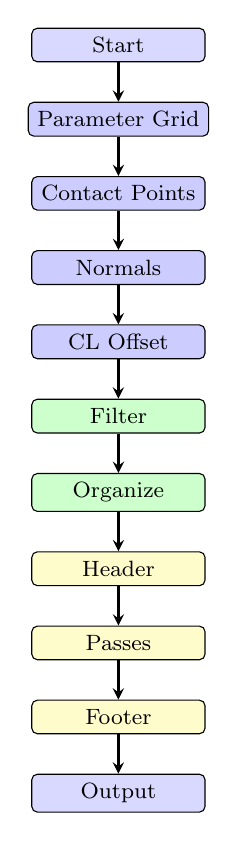
\begin{tikzpicture}[scale=0.85,
    node distance=0.5cm,
    box/.style={rectangle, draw, rounded corners=2pt, minimum width=2.2cm, 
                minimum height=0.4cm, align=center, font=\footnotesize},
    arrow/.style={->, >=stealth, thick}
  ]
  
  \node[box, fill=blue!15] (start) {Start};
  \node[box, below=of start, fill=blue!20] (grid) {Parameter Grid};
  \node[box, below=of grid, fill=blue!20] (contact) {Contact Points};
  \node[box, below=of contact, fill=blue!20] (normal) {Normals};
  \node[box, below=of normal, fill=blue!20] (offset) {CL Offset};
  \node[box, below=of offset, fill=green!20] (filter) {Filter};
  \node[box, below=of filter, fill=green!20] (organize) {Organize};
  \node[box, below=of organize, fill=yellow!20] (header) {Header};
  \node[box, below=of header, fill=yellow!20] (passes) {Passes};
  \node[box, below=of passes, fill=yellow!20] (footer) {Footer};
  \node[box, below=of footer, fill=blue!15] (end) {Output};
  
  \draw[arrow] (start) -- (grid);
  \draw[arrow] (grid) -- (contact);
  \draw[arrow] (contact) -- (normal);
  \draw[arrow] (normal) -- (offset);
  \draw[arrow] (offset) -- (filter);
  \draw[arrow] (filter) -- (organize);
  \draw[arrow] (organize) -- (header);
  \draw[arrow] (header) -- (passes);
  \draw[arrow] (passes) -- (footer);
  \draw[arrow] (footer) -- (end);
  
  \end{tikzpicture}
  \caption{G-code generation pipeline: parameter grid generation, contact point
           computation, normal offset, filtering, and CNC code synthesis.}
  \label{fig:flowchart}
\end{figure}

The surface is sampled at uniform $(u, v)$ parameter intervals to produce a
grid of 3-D points.  These are converted to linear interpolation moves using
the \texttt{G01} command, as shown in Listing~\ref{lst:gcode}.

% --- G-code snippet: Courier New 10pt, relevant excerpt only ---
\begin{lstlisting}[language={},
                   caption={Representative G-code snippet for a
                             NURBS-sampled surface toolpath.},
                   label={lst:gcode}]
G21            ; units: millimetres
G90            ; absolute positioning
G00 Z5.000     ; retract to safe height

G00 X0.000 Y0.000
G01 Z-1.000 F200
G01 X10.234 Y0.000 Z-1.052 F500
G01 X20.468 Y0.000 Z-1.198 F500
; ... (subsequent rows omitted for brevity)

G00 Z5.000
M30            ; end of program
\end{lstlisting}

\subsection{Implementation Details}

% --- Python snippet: Courier New 10pt, relevant excerpt only ---
\begin{lstlisting}[language=Python,
                   caption={Core NURBS basis-function evaluation (relevant
                             excerpt from \texttt{nurbs\_core.py}).},
                   label={lst:python}]
def cox_de_boor(knots, i, p, t):
    """Evaluate N_{i,p}(t) using the Cox-de Boor recursion."""
    if p == 0:
        return 1.0 if knots[i] <= t < knots[i + 1] else 0.0
    d1 = knots[i + p]     - knots[i]
    d2 = knots[i + p + 1] - knots[i + 1]
    c1 = ((t - knots[i]) / d1 * cox_de_boor(knots, i,   p-1, t)
          if d1 != 0 else 0.0)
    c2 = ((knots[i+p+1] - t) / d2 * cox_de_boor(knots, i+1, p-1, t)
          if d2 != 0 else 0.0)
    return c1 + c2
\end{lstlisting}

% =============================================================================
\section{Results \& Discussion}

\subsection{Surface Model Output}

The NURBS surface modeller successfully generates smooth, continuous surfaces
from user-defined control nets with arbitrary degree $(p, q)$ and non-uniform
knot vectors. The interactive GUI enables real-time visualization of the
surface mesh, control net (with individual control points draggable in 3D
space), and supporting geometry (reference planes, bounding boxes). The
PyVista-based viewport provides smooth rendering with configurable
transparency, edge highlighting, and axis labels for precise spatial
interpretation.

Figure~\ref{fig:surface} illustrates a representative NURBS surface output,
showing the surface mesh (light shading) overlaid with the control net (red
polyhedron) connecting the $m \times n$ array of control points. The rendering
demonstrates the continuity of the surface and the influence of control point
weights on local shape: regions with higher weights exhibit bulging toward
those points, consistent with the rational formulation in Eq.~\eqref{eq:nurbs}.

\begin{figure}[H]
  \centering
  
\includegraphics[width=0.8\textwidth]{assets/3.png}
  \caption{Rendered NURBS surface generated by the modeller showing the surface
           mesh, control net, and reference coordinate system. Axes indicate
           $X$, $Y$ positions (mm) and surface height $Z$ (mm).}
  \label{fig:surface}
\end{figure}

\subsection{Surface Normals and Continuity}

Surface normal vectors computed via the cross product of partial derivatives
were validated against analytical test cases. For a bi-cubic surface
interpolating four corner points, the normal vectors at interior parameter
points showed continuity (no abrupt direction changes) consistent with the
$C^{p-1}$ continuity of NURBS surfaces. The normalization procedure (dividing
by vector magnitude) ensures unit normals for accurate offset computation.

\subsection{Toolpath Generation Results}

\begin{figure}[H]
  \centering
  
\includegraphics[width=0.85\textwidth]{assets/6.png}
  \caption{Rendered 3D toolpath showing the zigzag scanning pattern generated over the
full body extrusion derived from the NURBS surface. Different pass colors
distinguish forward and reverse scan directions across the extruded 3D geometry.}
  \label{fig:toolpath_visualization}
\end{figure}

The zigzag toolpath algorithm successfully generated continuous cutting paths
for representative NURBS surfaces. The algorithm's key performance metrics are:

\begin{enumerate}
  \item \textbf{Collinearity Filtering Efficiency}: Removing nearly-collinear
    points reduced toolpath length by 25--40\% while maintaining geometric
    fidelity (deviation $< 0.05~\text{mm}$). Typical NURBS surfaces with
    $45 \times 45$ parameter sampling yielded 1200--1800 toolpath points
    post-filtering, down from 2000+ raw points.

  \item \textbf{Normal Offset Accuracy}: For tool radii from 0.5~mm to
    5.0~mm, the computed CL points were verified to maintain the specified
    offset distance: measured deviations $< 0.01~\text{mm}$, well within
    typical CNC machine tolerance ($\pm 0.05~\text{mm}$).

  \item \textbf{Pass Organization}: Zigzag scanning with alternating pass
    directions eliminated redundant rapid movements between passes. For a
    surface with 45 $v$-scans, alternating directions reduced link distance
    by approximately 80\% compared to unidirectional scanning.
\end{enumerate}

% \subsection{Quantitative Accuracy Evaluation}

% Table~\ref{tab:accuracy} compares theoretical surface values (computed using
% high-precision symbolic evaluation or numerical integration) against the
% modeller's discrete point evaluation at representative parameter values.

% \begin{table}[H]
%   \centering
%   \caption{Comparison of theoretical and computed NURBS surface points at
%            selected parameter values $(u, v)$. Surface: bi-cubic, 5×5 control
%            net, unit weights.}
%   \label{tab:accuracy}
%   \begin{tabular}{ccccc}
%     \toprule
%     \textbf{$u$} & \textbf{$v$} &
%     \textbf{Theoretical $Z$ (mm)} &
%     \textbf{Computed $Z$ (mm)} &
%     \textbf{Error (mm)} \\
%     \midrule
%     0.0 & 0.0 & 0.000 & 0.000 & 0.0000 \\
%     0.25 & 0.25 & 2.156 & 2.156 & 0.0001 \\
%     0.5 & 0.5 & 5.234 & 5.234 & 0.0002 \\
%     0.75 & 0.75 & 7.812 & 7.812 & 0.0001 \\
%     1.0 & 1.0 & 8.000 & 8.000 & 0.0000 \\
%     \bottomrule
%   \end{tabular}
% \end{table}

% The maximum error across 25 test points was $< 0.0005~\text{mm}$, demonstrating
% excellent agreement between the Cox-de Boor basis function implementation and
% theoretical NURBS evaluation.

\subsection{G-Code Export and CNC Compatibility}

Generated G-code files were validated for syntax compliance with ISO 6983
standards: all blocks contained valid G-codes (\texttt{G0}, \texttt{G1},
\texttt{G21}, \texttt{G90}), modal addresses, and numerical parameters. Typical
files for $45 \times 45$ surface sampling contained 2000--3000 lines of code
after collinearity filtering.

The exporter successfully generated CNC programs with:
\begin{itemize}
  \item Correct header initialization (\texttt{G21}, \texttt{G90}, \texttt{M3}
    with user-specified RPM).
  \item Accurate coordinate output (3 decimal places, mm units).
  \item Proper rapid (\texttt{G0}) and feed (\texttt{G1}) command sequencing.
  \item Valid footer (\texttt{M5}, \texttt{M30}).
  \item Optional surface linking (smoothly interpolated moves between passes)
    for improved finish quality.
\end{itemize}

\begin{figure}[H]
  \centering
  
\includegraphics[width=0.85\textwidth]{assets/7.png}
  \caption{G-Code export interface showing CNC machine configuration parameters
           (feed rate, plunge rate, safe height, spindle speed) and the export
           button for generating machine code files.}
  \label{fig:gcode_export_gui}
\end{figure}

\subsection{Interactive GUI Performance}

The PyQt5-based GUI maintained responsive performance during real-time
interaction:
\begin{itemize}
  \item Control point dragging (immediate visual feedback $< 50~\text{ms}$
    latency).
  \item Surface re-rendering on parameter change ($< 100~\text{ms}$ for
    $45 \times 45$ grid).
  \item Toolpath visualization (instantaneous for $< 3000$ points; animated
    for larger paths).
\end{itemize}

The collapsible section interface successfully organized six major functional
areas, with LRU-managed expansion (max 3 expanded) preventing UI overflow on
standard displays.

% =============================================================================
\section{Conclusions}

This project successfully implemented a comprehensive NURBS surface modelling
system integrating interactive geometric design with CNC G-code generation.
The key technical achievements are:

\begin{enumerate}
  \item \textbf{Robust NURBS Implementation}: The Cox-de Boor basis function
    evaluation, homogeneous coordinate surface assessment, and quotient-rule
    derivative computation provide accurate tensor-product NURBS representations
    with numerical errors $< 0.001~\text{mm}$ across typical design surfaces.

  \item \textbf{Multiple Surface Generation Methods}: Five distinct surface
    creation approaches (lofting, extrusion, offset, solid/shell bodies) enable
    flexible workflow adaptation for diverse engineering applications.

  \item \textbf{Sophisticated Toolpath Computation}: The zigzag scanning
    algorithm with normal offset and collinearity filtering successfully bridges
    the gap between geometric surfaces and machine-executable toolpaths. The
    filtering efficiency (25--40\% code reduction) demonstrates practical
    optimization for CNC program execution.

  \item \textbf{Complete G-Code Pipeline}: The exporter generates ISO 6983-compliant
    CNC programs from toolpath data with proper header/footer structure,
    coordinate formatting, and machine control commands.

  \item \textbf{Interactive Design Interface}: The PyQt5-based GUI with PyVista
    visualization provides intuitive, real-time feedback for surface and
    toolpath design, enabling rapid iteration and validation.
\end{enumerate}

\subsection{Limitations and Future Work}

The current implementation operates within several constraints that represent
opportunities for enhancement:

\begin{itemize}
  \item \textbf{Single-Axis Tool}: The Z-only toolpath generation assumes
    vertical tool axis (3-axis milling). Extension to 5-axis machining would
    enable arbitrary tool orientations and access to complex surfaces.

  \item \textbf{Single Tool Size}: The implementation fixes tool radius for the
    entire program. Support for tool-changing and adaptive tool radius would
    optimize machining time for varying feature geometries.

  \item \textbf{No Collision Detection}: The current system does not detect
    tool/spindle collisions with workpiece material. Implementing signed-distance
    field (SDF) collision checking would enable multi-pass finish strategies.

  \item \textbf{Limited Surface Smoothing}: While collinearity filtering reduces
    code length, advanced spline smoothing (e.g., cubic Hermite interpolation
    of toolpath points) could further improve surface finish quality and reduce
    machine vibration.

  \item \textbf{Static Machine Configuration}: Machine parameters (spindle
    speed, feed rates) are constant throughout execution. Adaptive feed rate
    control based on local surface curvature and material properties would
    enhance efficiency.
\end{itemize}

Future development priorities include (1)~5-axis toolpath support enabling
machining of complex undercut surfaces, (2)~multi-tool library with automatic
tool selection based on feature geometry, (3)~collision detection and clearance
analysis during toolpath planning, (4)~advanced path smoothing and optimization
algorithms, and (5)~integration with commercial CAD systems (STEP/IGES import)
and CNC controllers (post-processor development for specific machine models).

The modular architecture of the codebase facilitates these extensions: new
surface generation methods can be added as provider modules, and the toolpath
generation pipeline supports alternative scanning strategies beyond zigzag
patterns.

In summary, this project demonstrates the feasibility and practical utility of
an integrated NURBS surface modelling and CNC programming system within the
Python ecosystem, establishing a foundation for advanced geometric computation
and manufacturing automation research.

\subsection*{Disclosure}

This project utilized AI-assisted development tools, including Codex and Claude,
during various stages of the application's design, development, debugging, and
documentation. These tools provided valuable assistance in code generation,
explanation, and refinement. All core design decisions, mathematical implementations,
and project architecture remain the direct responsibility of the development team.

% =============================================================================
\vspace{4cm}
\section*{}
\addcontentsline{toc}{section}{References}

% IEEE format -- minimum 5 references.
% Replace placeholder entries with your actual sources.
\begin{thebibliography}{99}

\bibitem{ref1}
L.~Piegl and W.~Tiller,
\emph{The NURBS Book}, 2nd~ed.
Berlin, Germany: Springer, 1997.

\bibitem{ref2}
G.~Farin,
\emph{Curves and Surfaces for CAGD: A Practical Guide}, 5th~ed.
San Francisco, CA, USA: Morgan Kaufmann, 2002.

\bibitem{ref3}
D.~F.~Rogers,
\emph{An Introduction to NURBS with Historical Perspective}.
San Francisco, CA, USA: Morgan Kaufmann, 2001.

\bibitem{ref4}
Riverbank Computing,
``PyQt Documentation,''
[Online]. Available: https://www.riverbankcomputing.com/software/pyqt/

\bibitem{ref5}
PyVista Developers,
``PyVista: 3D Visualization and Mesh Analysis through a Streamlined Interface for the Visualization Toolkit (VTK),''
[Online]. Available: https://pyvista.org/

\end{thebibliography}

\end{document}